\section{Einleitung}

Der Versuch V14 umfasst die Anwendung des Verfahrens der Tomographie mittels
$\gamma -$Strahlung. Das Ziel des Versuches ist es die materielle Zusammensetzung
zwei bekannter, sowie einem unbekannten Objekt zu untersuchen.

\section{Theorie}

Die Tomgraphie ist ein bildgebendes Verfahren, welches auf dem Prinzip der Absorption
basiert. Dabei wird ein Objekt von $\gamma -$Strahlung, oder auch
Teilchen wie Elektronen oder Neutronen durchdrungen.
Die Anfangsintensität $I_0$ und Endintensität $I_{\symup{f}}$ werden vermessen, sodass die Absorptionskonstante
$\mu$ des durchdrungenen Materials bestimmt werden kann.\\

In dem Versuch wird ausschließlich $\gamma$-Strahlung verwendet. Diese wechselwirkt
mit Materie über drei Prozesse, der Photoeffekt, der Compton-Effekt und die Paarbildung.
Die Wirkungsquerschnitte der Prozesse sind abhängig von der Photonenenergie
der $\gamma$-Strahlung, sodass gilt $\sigma_i = \sigma_i\left(E_{\gamma}\right)$.
Eine exemplarische Darstellung der Wirkungsquerschnitte der drei Effekte ist in
Abb. \ref{fig:drei_effekte} anhand des Absorptionskoeffizienten von Blei dargestellt.

\begin{figure}[h]
  \centering
  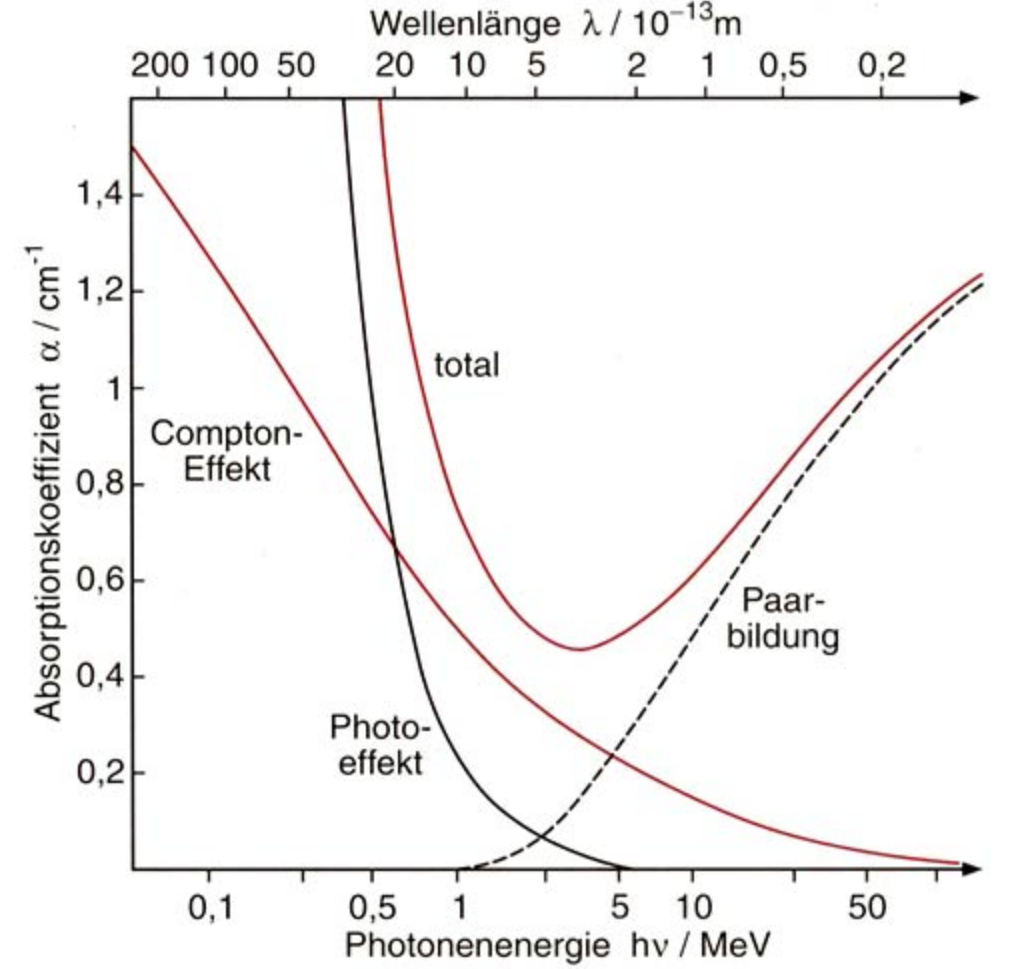
\includegraphics[width=0.7\textwidth]{Pics/drei_effekte.png}
  \caption{Beiträge von Photoeffekt, Compton-Effekt und Paarbildung zum Absorptionskoeffizienten
  von Blei in Abhängigkeit von der Photonenenergie.\cite{drei_effekte}}
  \label{fig:drei_effekte}
\end{figure}

Die Intensitäten der materialdurchdringenden Photonen hängen über einen exponentiellen Zusammenhang mit der
Absorptionskonstate und der Materialdicke $d$ zusammen.

\begin{equation}
  I_{\symup{f}} = I_0 \exp{-\sum_i\mu\cdot d_i}
  \label{eqn:absorption}
\end{equation}

Die Absorptionskonstate ist materialspezifisch, weshalb aufgrund ihres Wertes
auf das Material zurückgeschlossen werden kann.
Das einmaligen Durchführen des Verfahren gibt lediglich einen Eindruck von einem
Querschnittes des Objektes. Deshalb ist eine mehrfach Ausführung
mit verschiedenen Durchdringungsrichtungen notwendig, um das Gesamtobjekt zu vermessen.

Die Gleichung \eqref{eqn:absorption} kann umgestellt werden, sodass ein
Gleichungssystem der Form:

\begin{equation}
  \underline{\underline{A}} \cdot \vec{\mu} = \vec{I}
  \label{eqn:LGS}
\end{equation}

In dem Versuch wird ein $3 \times 3 \times 3$ Würfel untersucht.
Deshalb ist die Dicke der einzelnen Würfel $d_i$ gleich $d = \SI{1}{\centi\meter}$
für alle Einheitswürfel.
Das bedeutet, dass es insgesamt neun verschiedene Absorptionskonstanten $\mu_1, \mu_2, ... , \mu_9$
in einer Ebene des Würfels vorliegen. Dementsprechend werden mindestend neun
verschiedene Projektionen benötigt, um das Gleichungssytem \eqref{eqn:LGS}
zu lösen. Das Messverfahren wird durch eine Überbestimmung des
Gleichungssytems erhöht, weshalb anstelle der nötigen neun Projektionen
zwölf Projektionen gewählt werden.
Eine Darstellung der gewählten Projektionen ist in Abb. \ref{fig:projektionen}
zu sehen.

\begin{figure}[h]
  \centering
  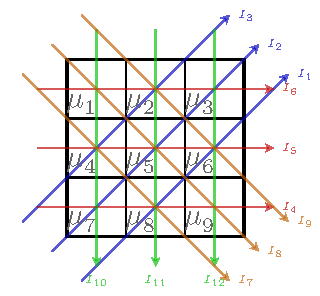
\includegraphics[width=0.7\textwidth]{Pics/tikz-Projektionen.pdf}
  \caption{Schematische Darstellung der zwölf verwendeten Projektionen $I_1$ -- $I_{12}$.\cite{LuckyJosh}}
  \label{fig:projektionen}
\end{figure}

Die gewählten Projektionen erzeugen ein Gleichungssystem der Form:

\begin{align}
    d \cdot
    \begin{pmatrix}
      0 & 0 & 0 & 0 & 0 & \sqrt{2} & 0 & \sqrt{2} & 0 \\
      0 & 0 & \sqrt{2} & 0 & \sqrt{2} & 0 & \sqrt{2} & 0 & 0 \\
      0 & \sqrt{2} & 0 & \sqrt{2} & 0 & 0 & 0 & 0 & 0 \\
      0 & 0 & 0 & 0 & 0 & 0 & 1 & 1 & 1 \\
      0 & 0 & 0 & 1 & 1 & 1 & 0 & 0 & 0 \\
      1 & 1 & 1 & 0 & 0 & 0 & 0 & 0 & 0 \\
      0 & 0 & 0 & \sqrt{2} & 0 & 0 & 0  & \sqrt{2} & 0 \\
      \sqrt{2} & 0 & 0 & 0 & \sqrt{2} & 0 & 0 & 0 & \sqrt{2} \\
      0 & \sqrt{2} & 0 & 0 & 0  & \sqrt{2} & 0 & 0 & 0\\
      1 & 0 & 0 & 1 & 0 & 0 & 1 & 0 & 0 \\
      0 & 1 & 0 & 0 & 1 & 0 & 0 & 1 & 0 \\
      0 & 0 & 1 & 0 & 0 & 1 & 0 & 0 & 1 \\
    \end{pmatrix}
    \cdot
    \begin{pmatrix}
      \mu_1 \\
      \mu_2 \\
      \mu_3 \\
      \mu_4 \\
      \mu_5 \\
      \mu_6 \\
      \mu_7 \\
      \mu_8 \\
      \mu_9 \\
      \mu_{10} \\
      \mu_{11} \\
      \mu_{12} \\
    \end{pmatrix}
    =
    \begin{pmatrix}
      I_1 \\
      I_2 \\
      I_3 \\
      I_4 \\
      I_5 \\
      I_6 \\
      I_7 \\
      I_8 \\
      I_9 \\
      I_{10} \\
      I_{11} \\
      I_{12} \\
    \end{pmatrix}.
    \label{eqn:LGS_ausgeschrieben}
\end{align}

Aufrund der Überbestimmtheit von \eqref{eqn:LGS_ausgeschrieben} wird die
"Methode der kleinsten Quadrate" verwendet, wodurch \eqref{eqn:LGS_ausgeschrieben}
in eine Normalengleichung der Form $\left(\underline{\underline{A}}^T\underline{\underline{A}}\right)
\cdot \vec{\mu} = \left(\underline{\underline{A}}^T\cdot\vec{I}\right)$ überführt wird.
Umgestellt nach $\vec{\mu}$ ergibt:

\begin{equation}
  \vec{\mu} = \left(\underline{\underline{A}}^T\underline{\underline{A}}\right)^{-1}
  \underline{\underline{A}}^T\cdot \vec{I}.
  \label{eqn:mu_umgestellt}
\end{equation}

Die Varianz des Vektors $\vec{I}$ ist durch eine Diagonalmatrix gegeben (vgl. \eqref{eqn:kovarianz_I}).

\begin{equation}
  \symup{V}[\vec{I}] = \text{diag}\left(\sigma_{I_1}^2, \sigma_{I_2}^2, ... , \sigma_{I_{12}}^2\right)
  \label{eqn:kovarianz_I}
\end{equation}

Daraus ergibt sich die Kovarianzmatrix von $\vec{\mu}$ zu:

\begin{equation}
  \symup{V}[\vec{\mu}] = \left(\underline{\underline{A}}^T \symup{V}^{-1}[\vec{I}] \underline{\underline{A}}\right)^{-1}.
  \label{eqn:kovarianz_mu}
\end{equation}

Damit muss $\vec{\mu}$ umgeschrieben werden zu:

\begin{equation}
  \vec{\mu} = \symup{V}[\vec{\mu}] \underline{\underline{A}}^T \symup{V}^{-1}[\vec{I}] \cdot \vec{I}.
  \label{eqn:mu}
\end{equation}

\section{Durchführung}

Die Durchführung des Versuches benötigt eine $\gamma$-Strahlungsquelle,
einen Szintillationsdetektor, einen Vielkanalanalysator, Bleiabschrimungen und
einen Computer, der die Daten des Vielkanalanalysators aufnimmt und mit geeigneter
Software verarbeitet.
Eine Abbildung des verwendeten Aufbaus ist in \ref{fig:Aufbau} dargestellt.
Auf der Abbildung fehlen die Bleiabschirmungen, die geeignet den Versuch positioniert werden,
sodass die Sicherheit vor Streuustrahlung gewährleistet ist.\\

Als $\gamma$-Strahlungsquelle wurde das Caesium-Isotop 137 $(\ce{^137Cs})$
verwendet, welches $\gamma$-Strahlung mit einer Energie von $E_{\gamma}\approx \SI{0.6617}{\mega\eV}$
besitzt. Die Photonenenergie ist kleiner als die Energie, bei der der Effekt
der Parrbildung auftritt. Damit sind die beiden relevanten Prozesse der Photonenwechselwirkung
mit Materie der Photoeffekt und der Compton-Effekt.\\

Die untersuchten Objekte sind die bereits erwähnten $3 \times 3 \times 3$ Würfel,
die aus insgesamt 27 Einheitswürfel aufgebaut sind.
Insgesamt werden drei Proben, sowie eine Referenzprobe untersucht.
Die Referenzprobe $\symup{P}_1$ ist ein $3 \times 3 \times 3$ Würfel, der nur aus der Ummantelung
besteht und dessen Einheitswürfel aus Luft bestehen. Dieser dient dazu den
Wert der eingehenden Anfangsintensität $I_0$ zu bestimmen und es werden für diese
Probe lediglich die Projektionen $I_2, I_3 und I_6$ ausgemessen.\\
Weiterhin gibt es zwei Proben aus bekannten Materialien ($\symup{P}_2:$ Aluminium und $\symup{P}_3:$ Blei)
und eine unbekannte Probe $\symup{P}_4$. Die Einheitswürfel von $\symup{P}_4$ sind
entweder aus Blei oder aus Aluminium, aber die Zusammensetzung ist a priori nicht
bekannt und gilt als zu ermitteln.
Für diese Proben sind alle zwölf Projektionen auszumessen.\\

Zu Beginn wird das Computerprogramm gestartet und auf seine Funktionsfähigkeit
überprüft. Danach wird die Proben $\symup{P}_2$ in die in Abb. \ref{fig:aufbau}
dargestellt Halterung eingebracht und so ausgerichtet, dass die erste Projektion
$I_1$ von dem Photonenstrahl hin zum Detektor realisiert wird.
Die weiteren Projektionen können durch Drehen und Kalibrieren der Halterung eingestellt
werden.
Die anderen Proben werden im gleichen Verfahren in der Reihenfolge $\symup{P}_3,
symup{P}_1$ und $\symup{P}_4$ ausgemessen.

Bei den Proben $\symup{P}_1$ und $\symup{P}_4$ werden solange Messwert genommen,
bis in einem Bereich von 10 bis 14 Kanälen um den Peak herum im Vielkanalanalysator
$\num{12500}$ bis $\num{15000}$ Ereignisse sind.

Die Proben $\symup{P}_2$ und $\symup{P}_3$ werden nur solange vermessen, bis die
statistische Unsicherheit in 5 bis 7 Kanälen um den Peak herum
$\leq 3\%$ ist. Dies entspricht ca. $\num{1200}$ Ereignissen,
da $\frac{\sqrt{N}}{N} = 3\%$ für $N = \num{1200}$ realisiert ist.
Dabei ist $N$ die Anzahl der Ereignisse.

\begin{figure}[h]
  \centering
  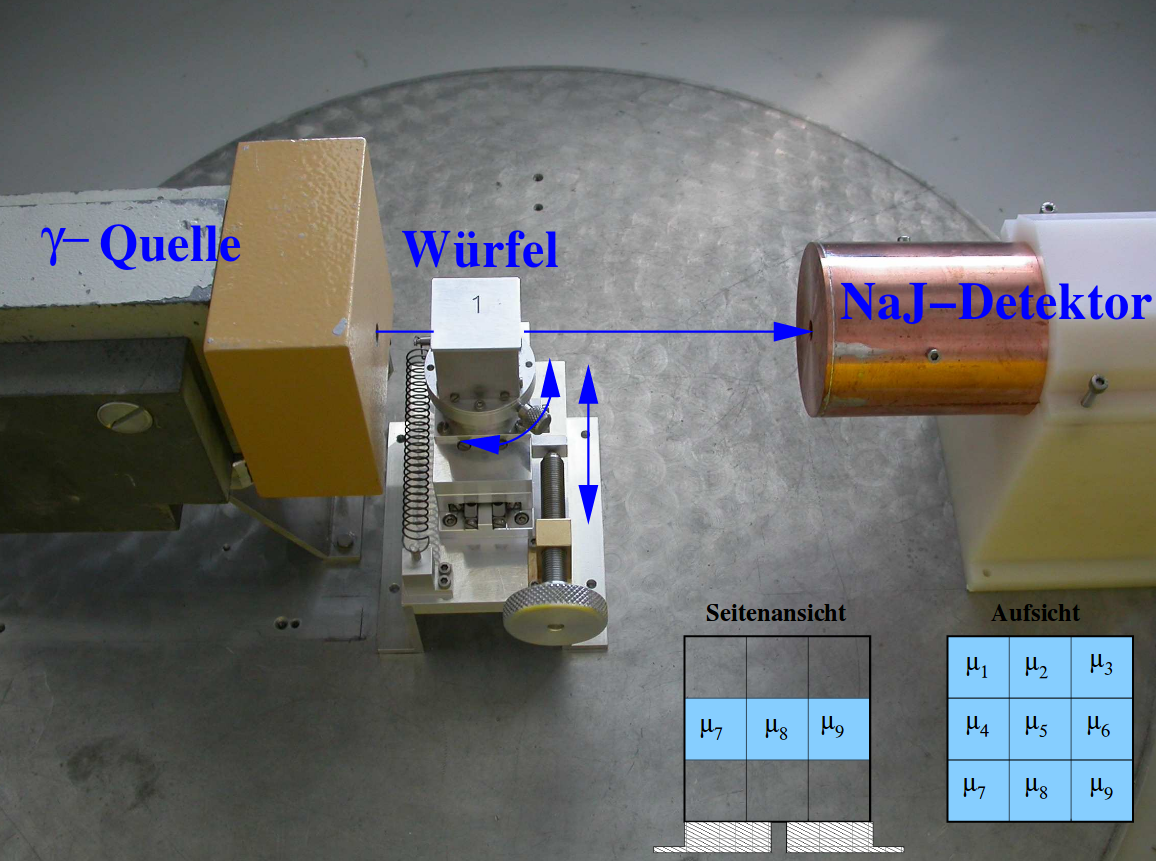
\includegraphics[width=0.8\textwidth]{Pics/Aufbau.png}
  \caption{Verwendeter Veruschsaufbau. Nahaufnahme der Messaparatur.\cite{anleitung}}
  \label{fig:aufbau}
\end{figure}

\newpage
